\documentclass[12pt]{article}
\usepackage[utf8]{inputenc}
\usepackage{graphicx}
\usepackage{subcaption}
\usepackage{amsmath}
\usepackage{fancyhdr}
\usepackage{geometry}
\usepackage{dirtytalk}
\usepackage[english]{babel}
\usepackage{csquotes}
\usepackage{hyperref}
\usepackage{listings}
\lstset{
    language=C,
    basicstyle=\ttfamily,
    numberstyle=\tiny,
    frame=single,
    breaklines=true,
}

\begin{document}
\begin{titlepage}
\begin{center}
    
\includegraphics[width=0.3\textwidth]{image.png} \\[0.2cm]
    
    \textbf{MINISTRY OF EDUCATION, CULTURE AND RESEARCH \\
    OF THE REPUBLIC OF MOLDOVA} \\[0.3cm]
    
    \textbf{Technical University of Moldova \\
    Faculty of Computers, Informatics and Microelectronics \\
    Department of Software and Automation Engineering} \\[2cm]
    
    \textbf{Postoronca Dumitru FAF-233}\\[0.5cm]
    
    \Huge \textbf{Report} \\[0.5cm]
    
    \large Laboratory Work №5\\[0.5cm]
    
    \textbf{on Minimum Spanning Trees: Prim and Kruskal} \\[3cm]
    
    \begin{flushright}
        \textit{Checked by:} \\
        \textbf{Fistic Cristofor}, \textit{university assistant} \\
        DISA, FCIM, UTM
    \end{flushright}
    
    \vfill
    
    Chi{\c{s}}in{\u{a}}u -- 2024
\end{center}
\end{titlepage}

\newpage
\setcounter{page}{1}
\pagestyle{fancy}
\fancyhf{}
\rhead{\thepage}
\lhead{FAF-233 Postoronca Dumitru; Laboratory Work №5}

\section*{Conditions of the Task}
In this laboratory work we explore greedy algorithms for constructing minimum spanning trees (MST) in a connected, weighted, undirected graph. The objectives are:
\begin{enumerate}
    \item Study the greedy design technique as applied to MST.
    \item Implement Prim's and Kruskal's algorithms in a programming language.
    \item Empirically analyze and compare their performance on graphs of varying size and density.
    \item Present the data graphically and draw conclusions on algorithmic efficiency.
\end{enumerate}

\section*{Input Data}
Graphs are generated programmatically with the following parameters:
\begin{itemize}
  \item Number of nodes $N$: low (100), medium (500), high (1000).
  \item Graph density $d$: sparse ($d=0.1$), medium ($d=0.4$), dense ($d=0.8$).
  \item Edge weights: integers uniformly drawn from [1, 100].
\end{itemize}
Each test case runs both algorithms on identical random graphs to ensure fair comparison.

\clearpage
\section*{Metrics in Algorithm Analysis}
We measure:
\begin{itemize}
  \item Execution time (in milliseconds) for building the MST.
  \item Number of edge-comparison operations.
\end{itemize}
Tests are repeated 10 times per configuration and averaged to mitigate randomness.

\section*{Algorithms Implementation}
Both algorithms are implemented in Python using adjacency lists. The implementations include:
\begin{itemize}
  \item \textbf{Prim's Algorithm:} Using a binary min-heap (priority queue) to select the next minimum edge.
  \item \textbf{Kruskal's Algorithm:} Sorting all edges then applying Union-Find with path compression.
\end{itemize}
Detailed code listings are available in the Appendix.

\section*{Results}
Average runtimes for varying $N$ and density $d$ are shown below.

\begin{figure}[h]
    \centering
    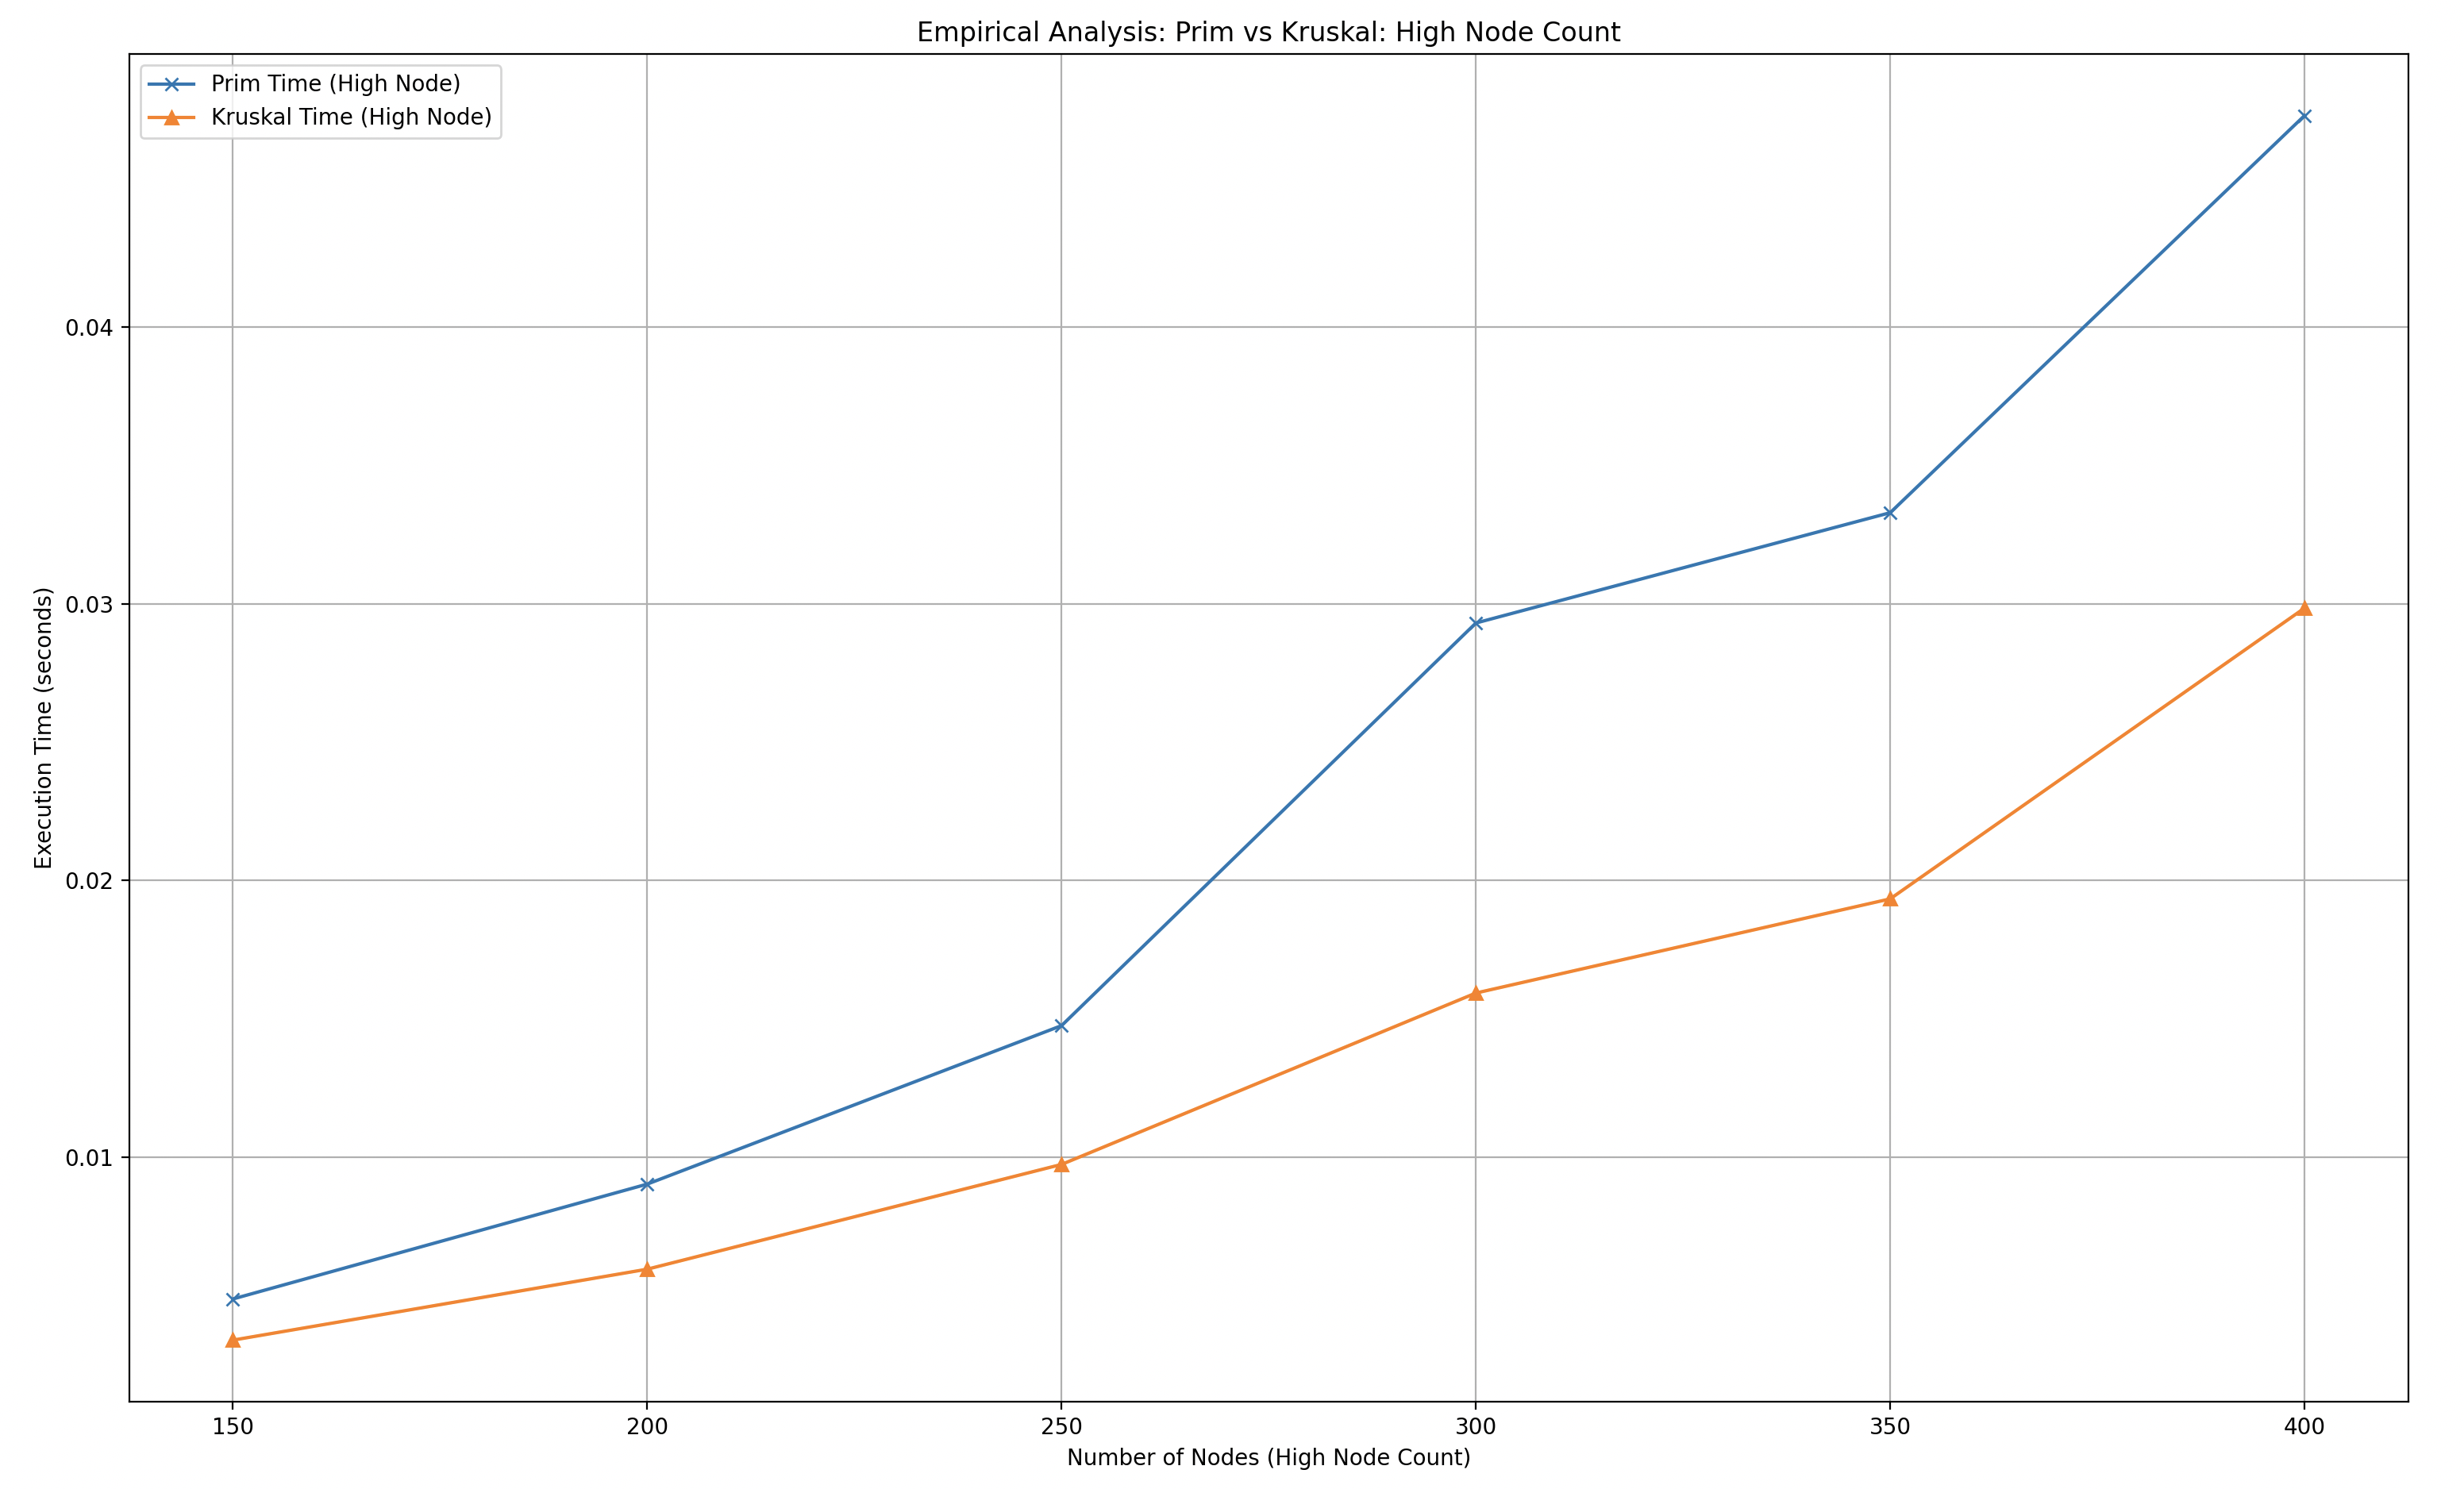
\includegraphics[width=0.9\textwidth]{images/more_nodes.png}
    \caption{Runtime comparison on dense graphs ($d=0.8$)}
    \label{fig:dense}
\end{figure}

\begin{figure}[h]
    \centering
    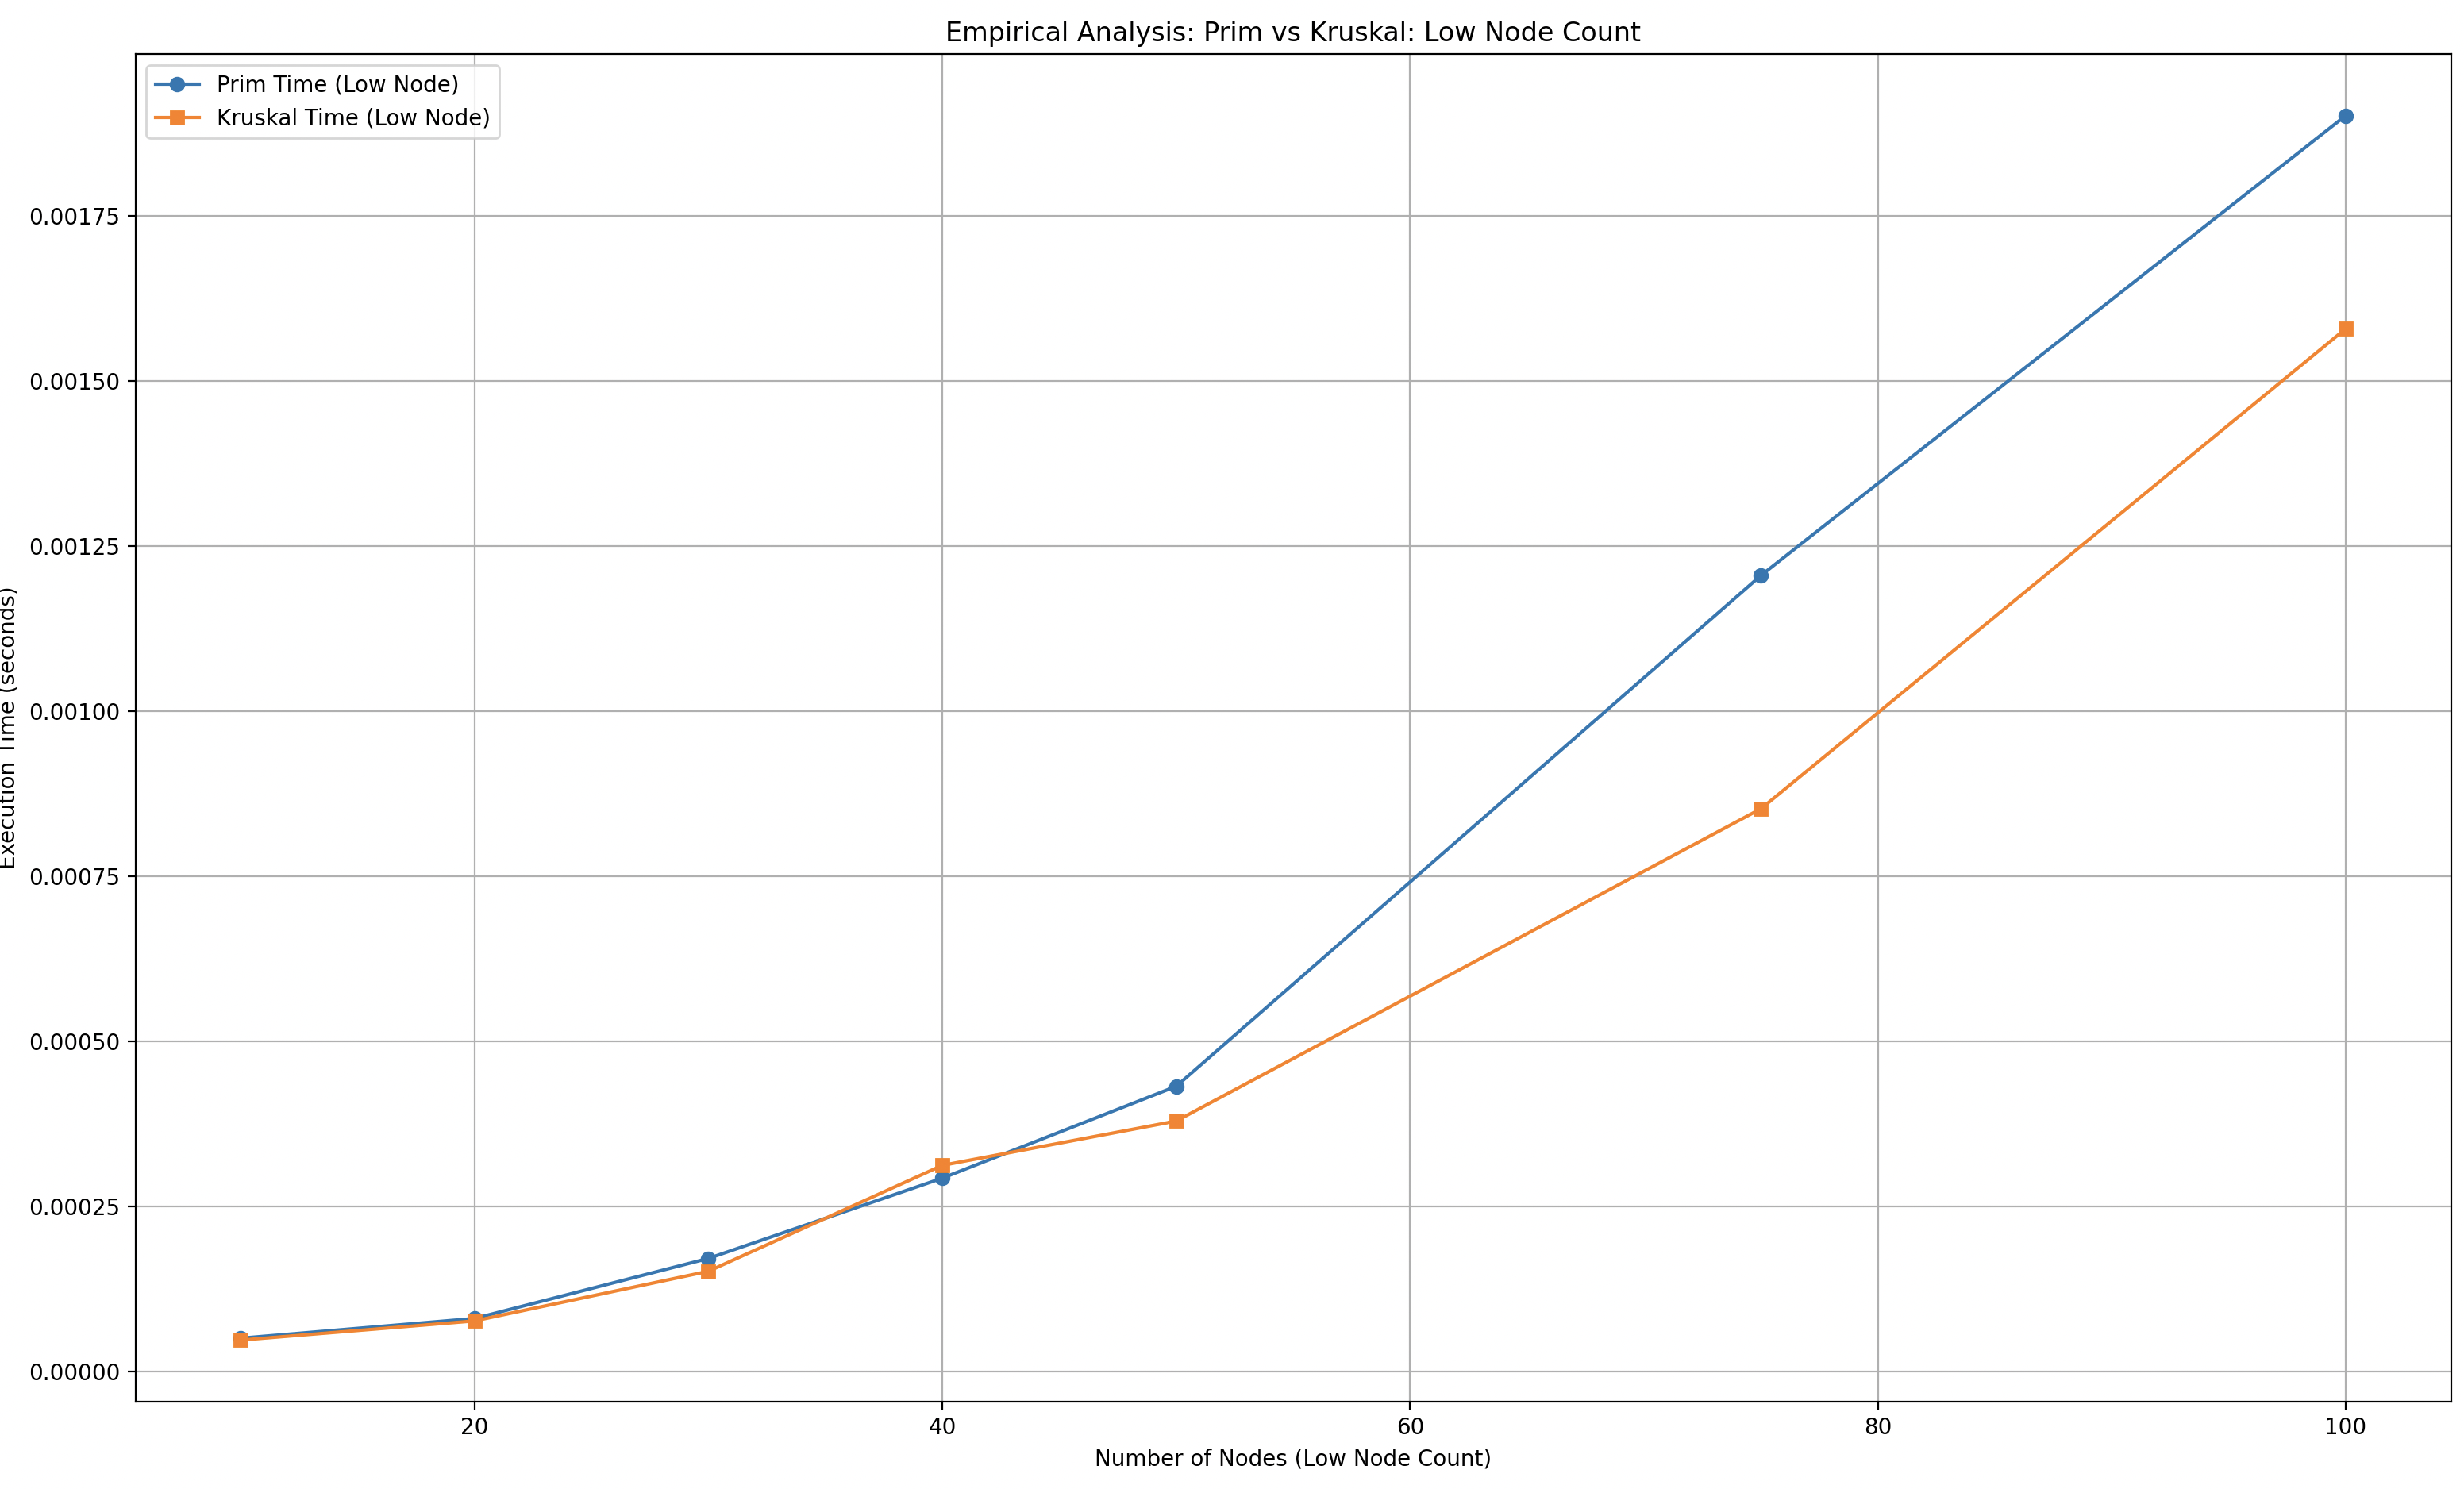
\includegraphics[width=0.9\textwidth]{images/less_nodes.png}
    \caption{Runtime comparison on sparse graphs ($d=0.1$)}
    \label{fig:sparse}
\end{figure}

\clearpage
\section*{Graphical Visualization}
An interactive web-based tool was developed to illustrate algorithm execution step-by-step:
\begin{itemize}
  \item Select Prim or Kruskal.
  \item Choose source and destination nodes for path extraction (in addition to MST construction).
  \item View real-time logs of edge selection and acceptance/rejection.
\end{itemize}
The tool is accessible at \url{https://lab4-5visualising.vercel.app/}.

\clearpage
\begin{figure}[h]
    \centering
    \begin{subfigure}{0.7\textwidth}
      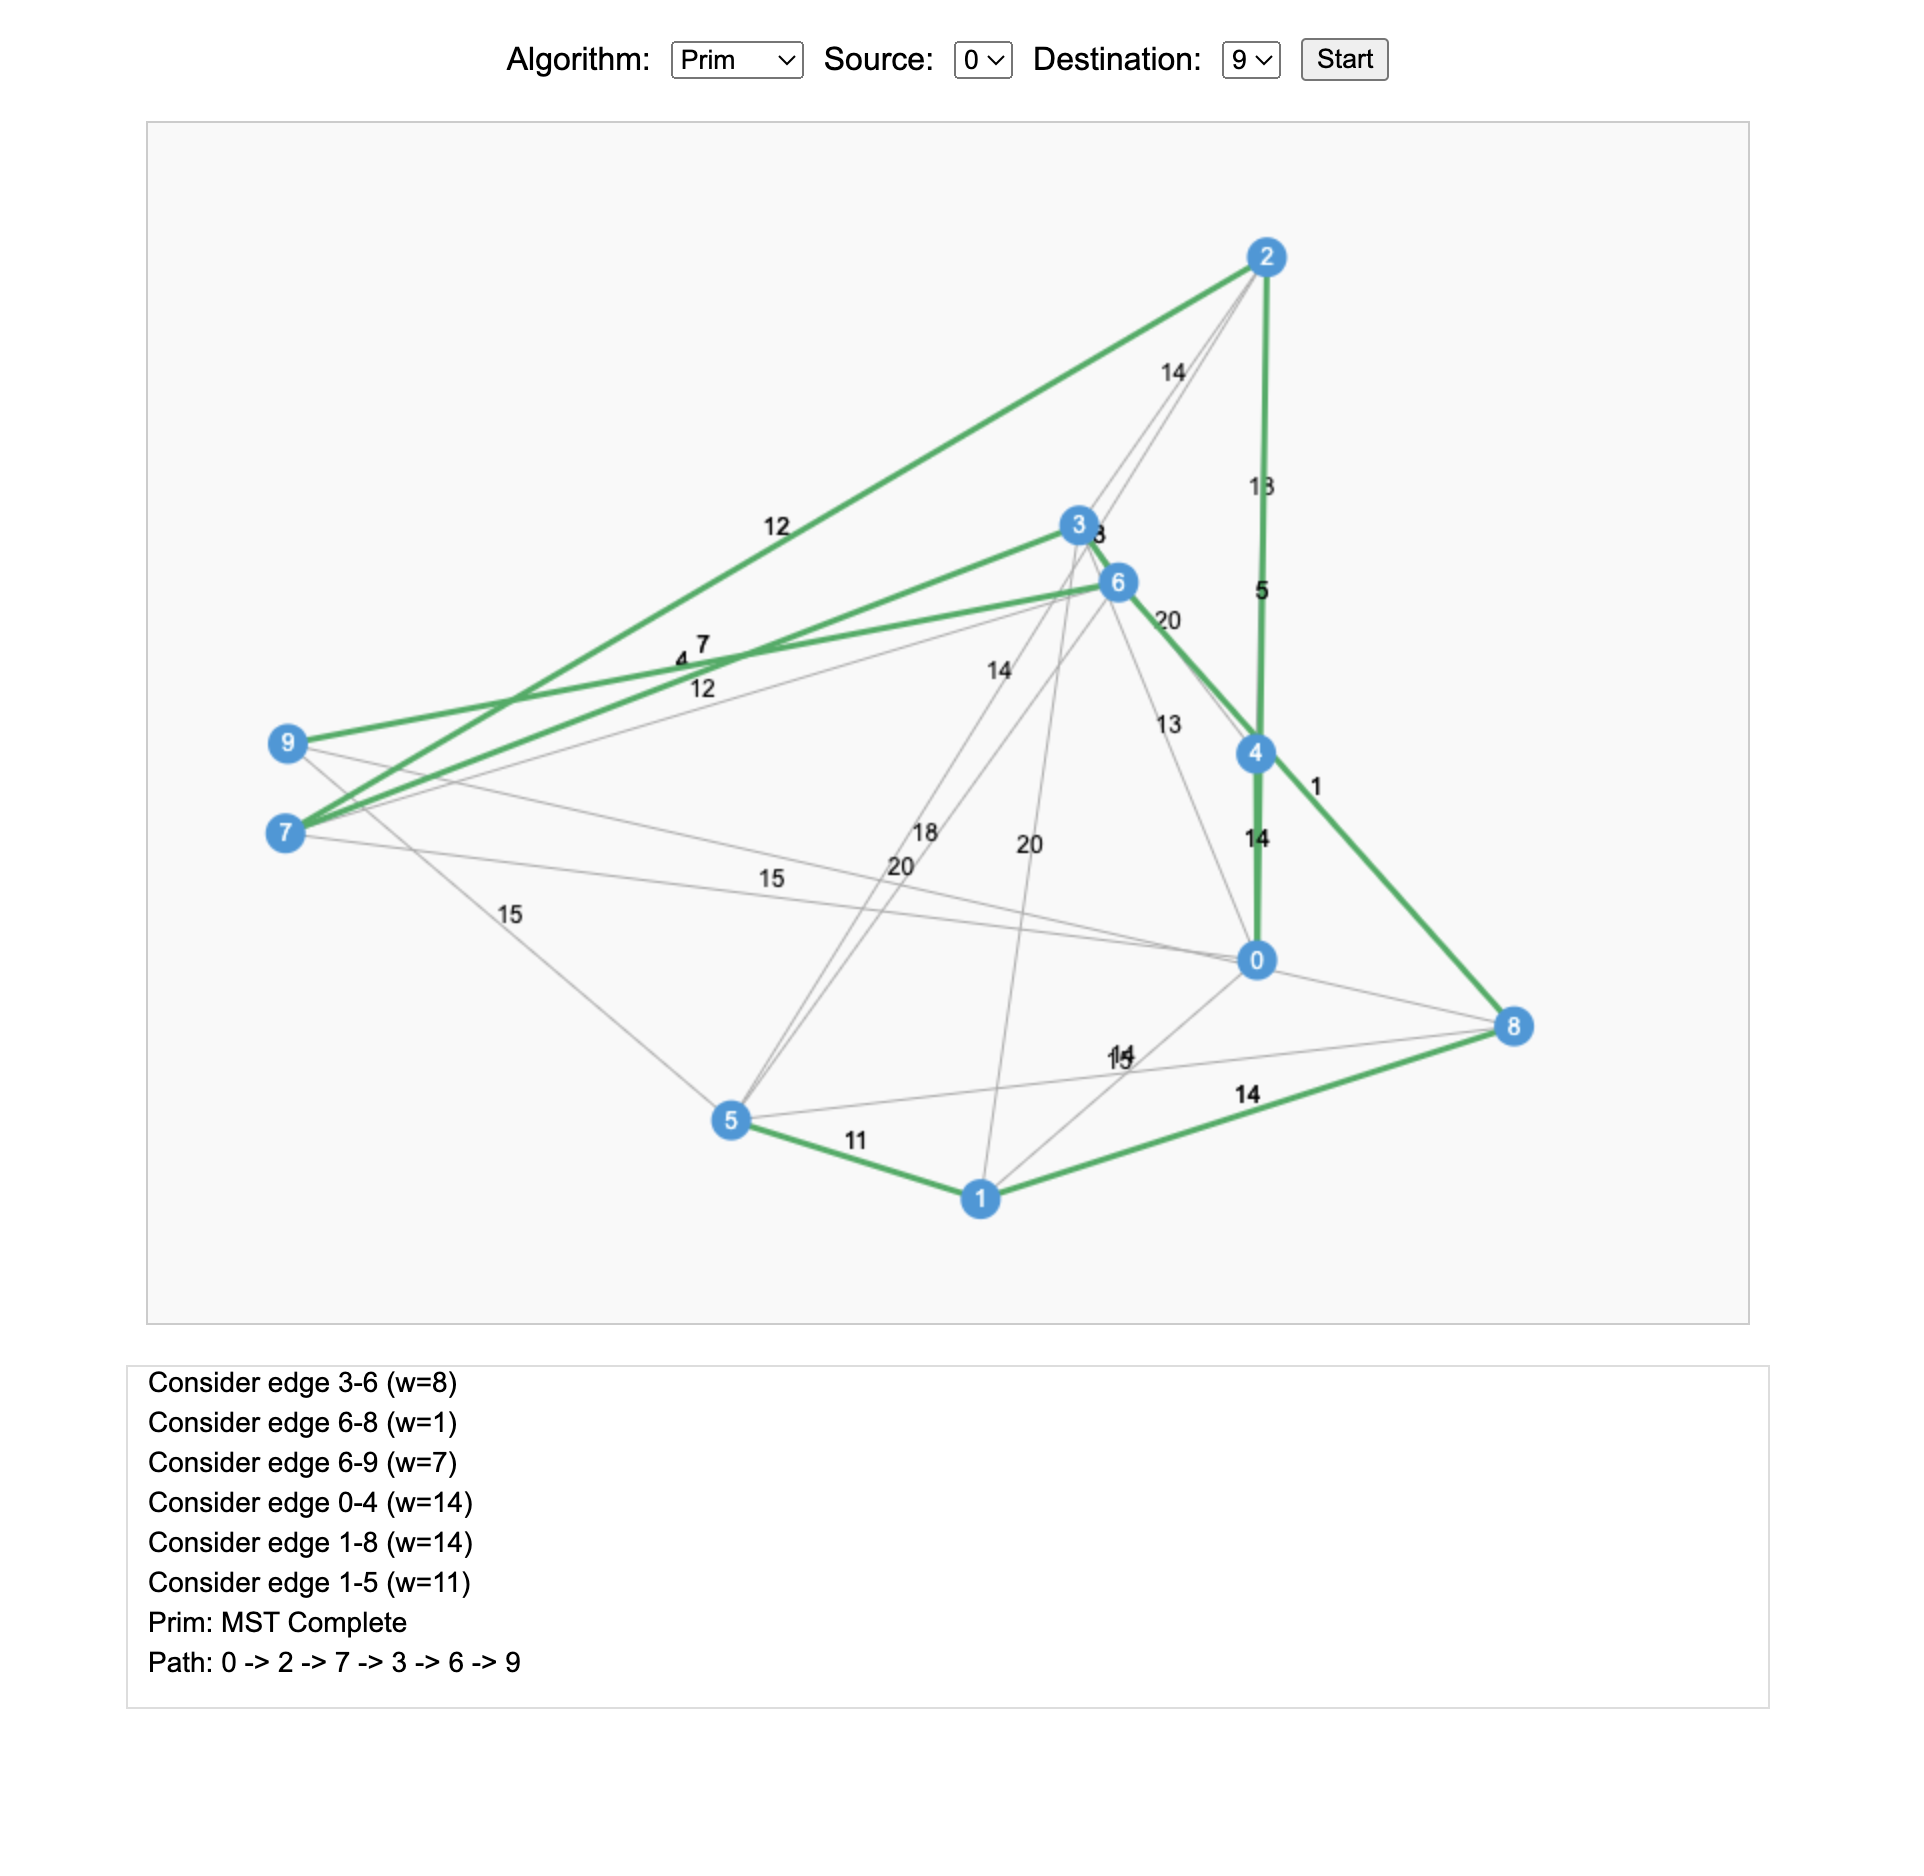
\includegraphics[width=\linewidth]{images/vis_prim.png}
      \caption{Prim's algorithm in action}
    \end{subfigure}\hfill
    \begin{subfigure}{0.7\textwidth}
      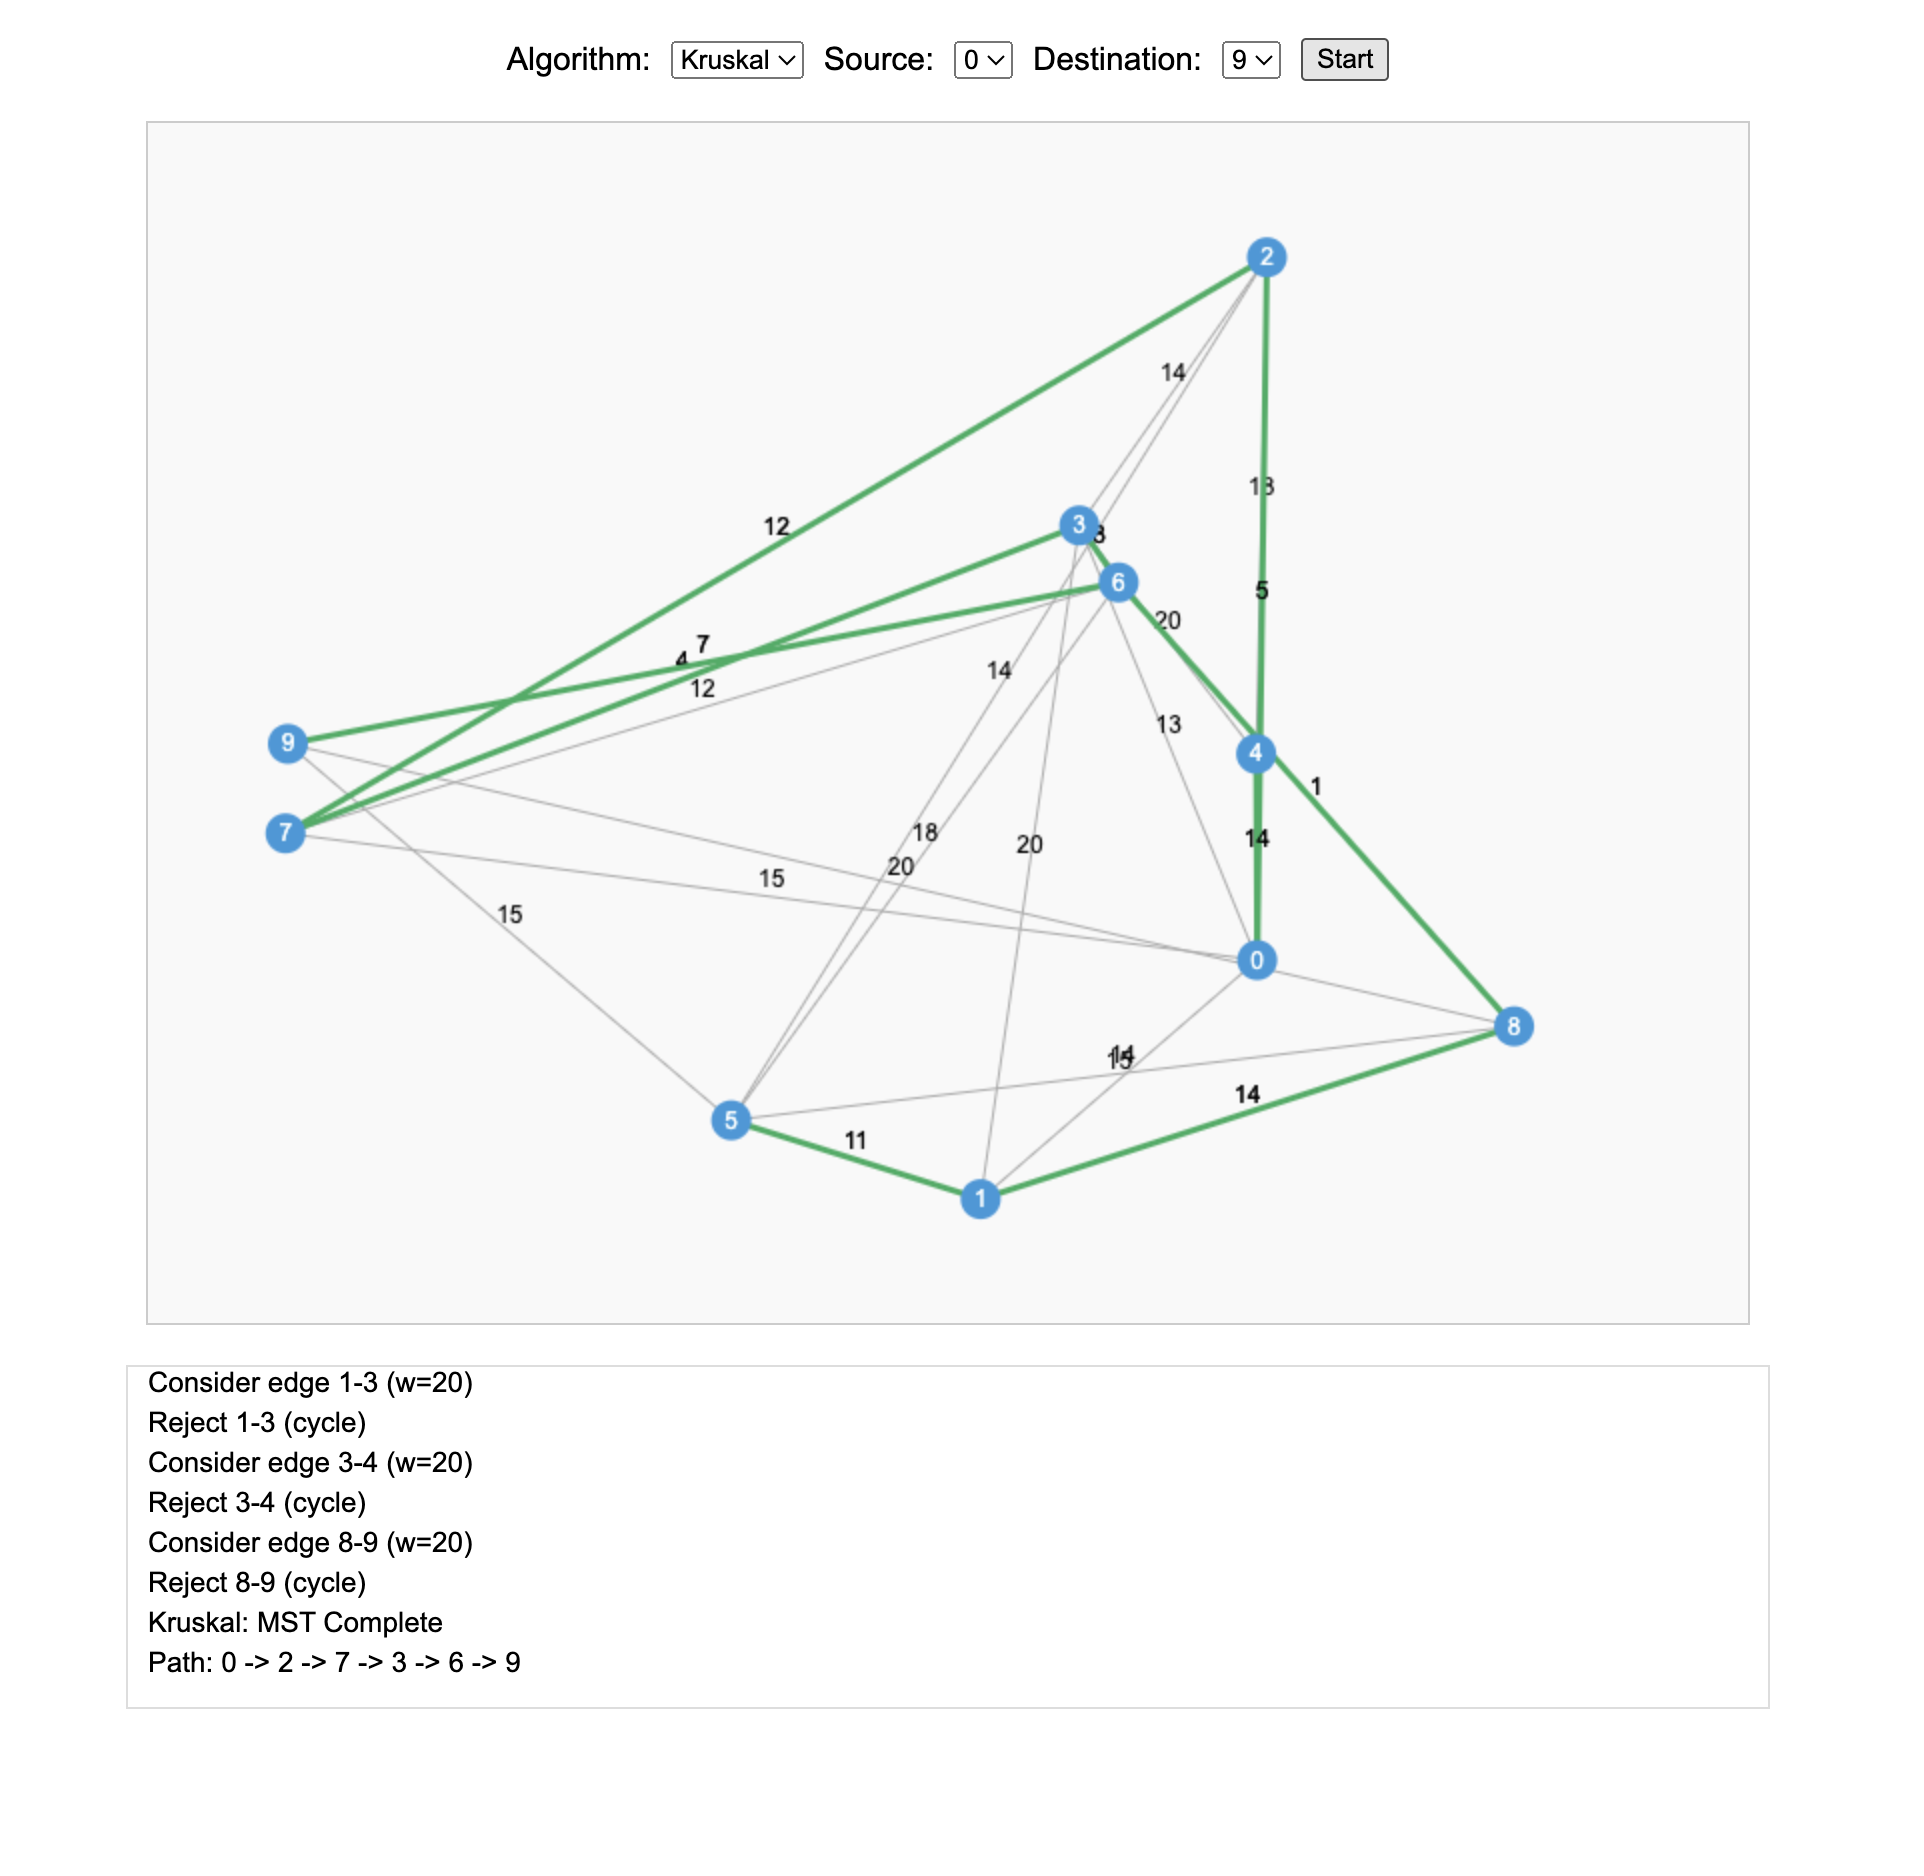
\includegraphics[width=\linewidth]{images/vis_kruskal.png}
      \caption{Kruskal's algorithm in action}
    \end{subfigure}
    \caption{Snapshots of the MST Visualizer UI}
    \label{fig:ui}
\end{figure}

\begin{figure}[h]
    \centering
    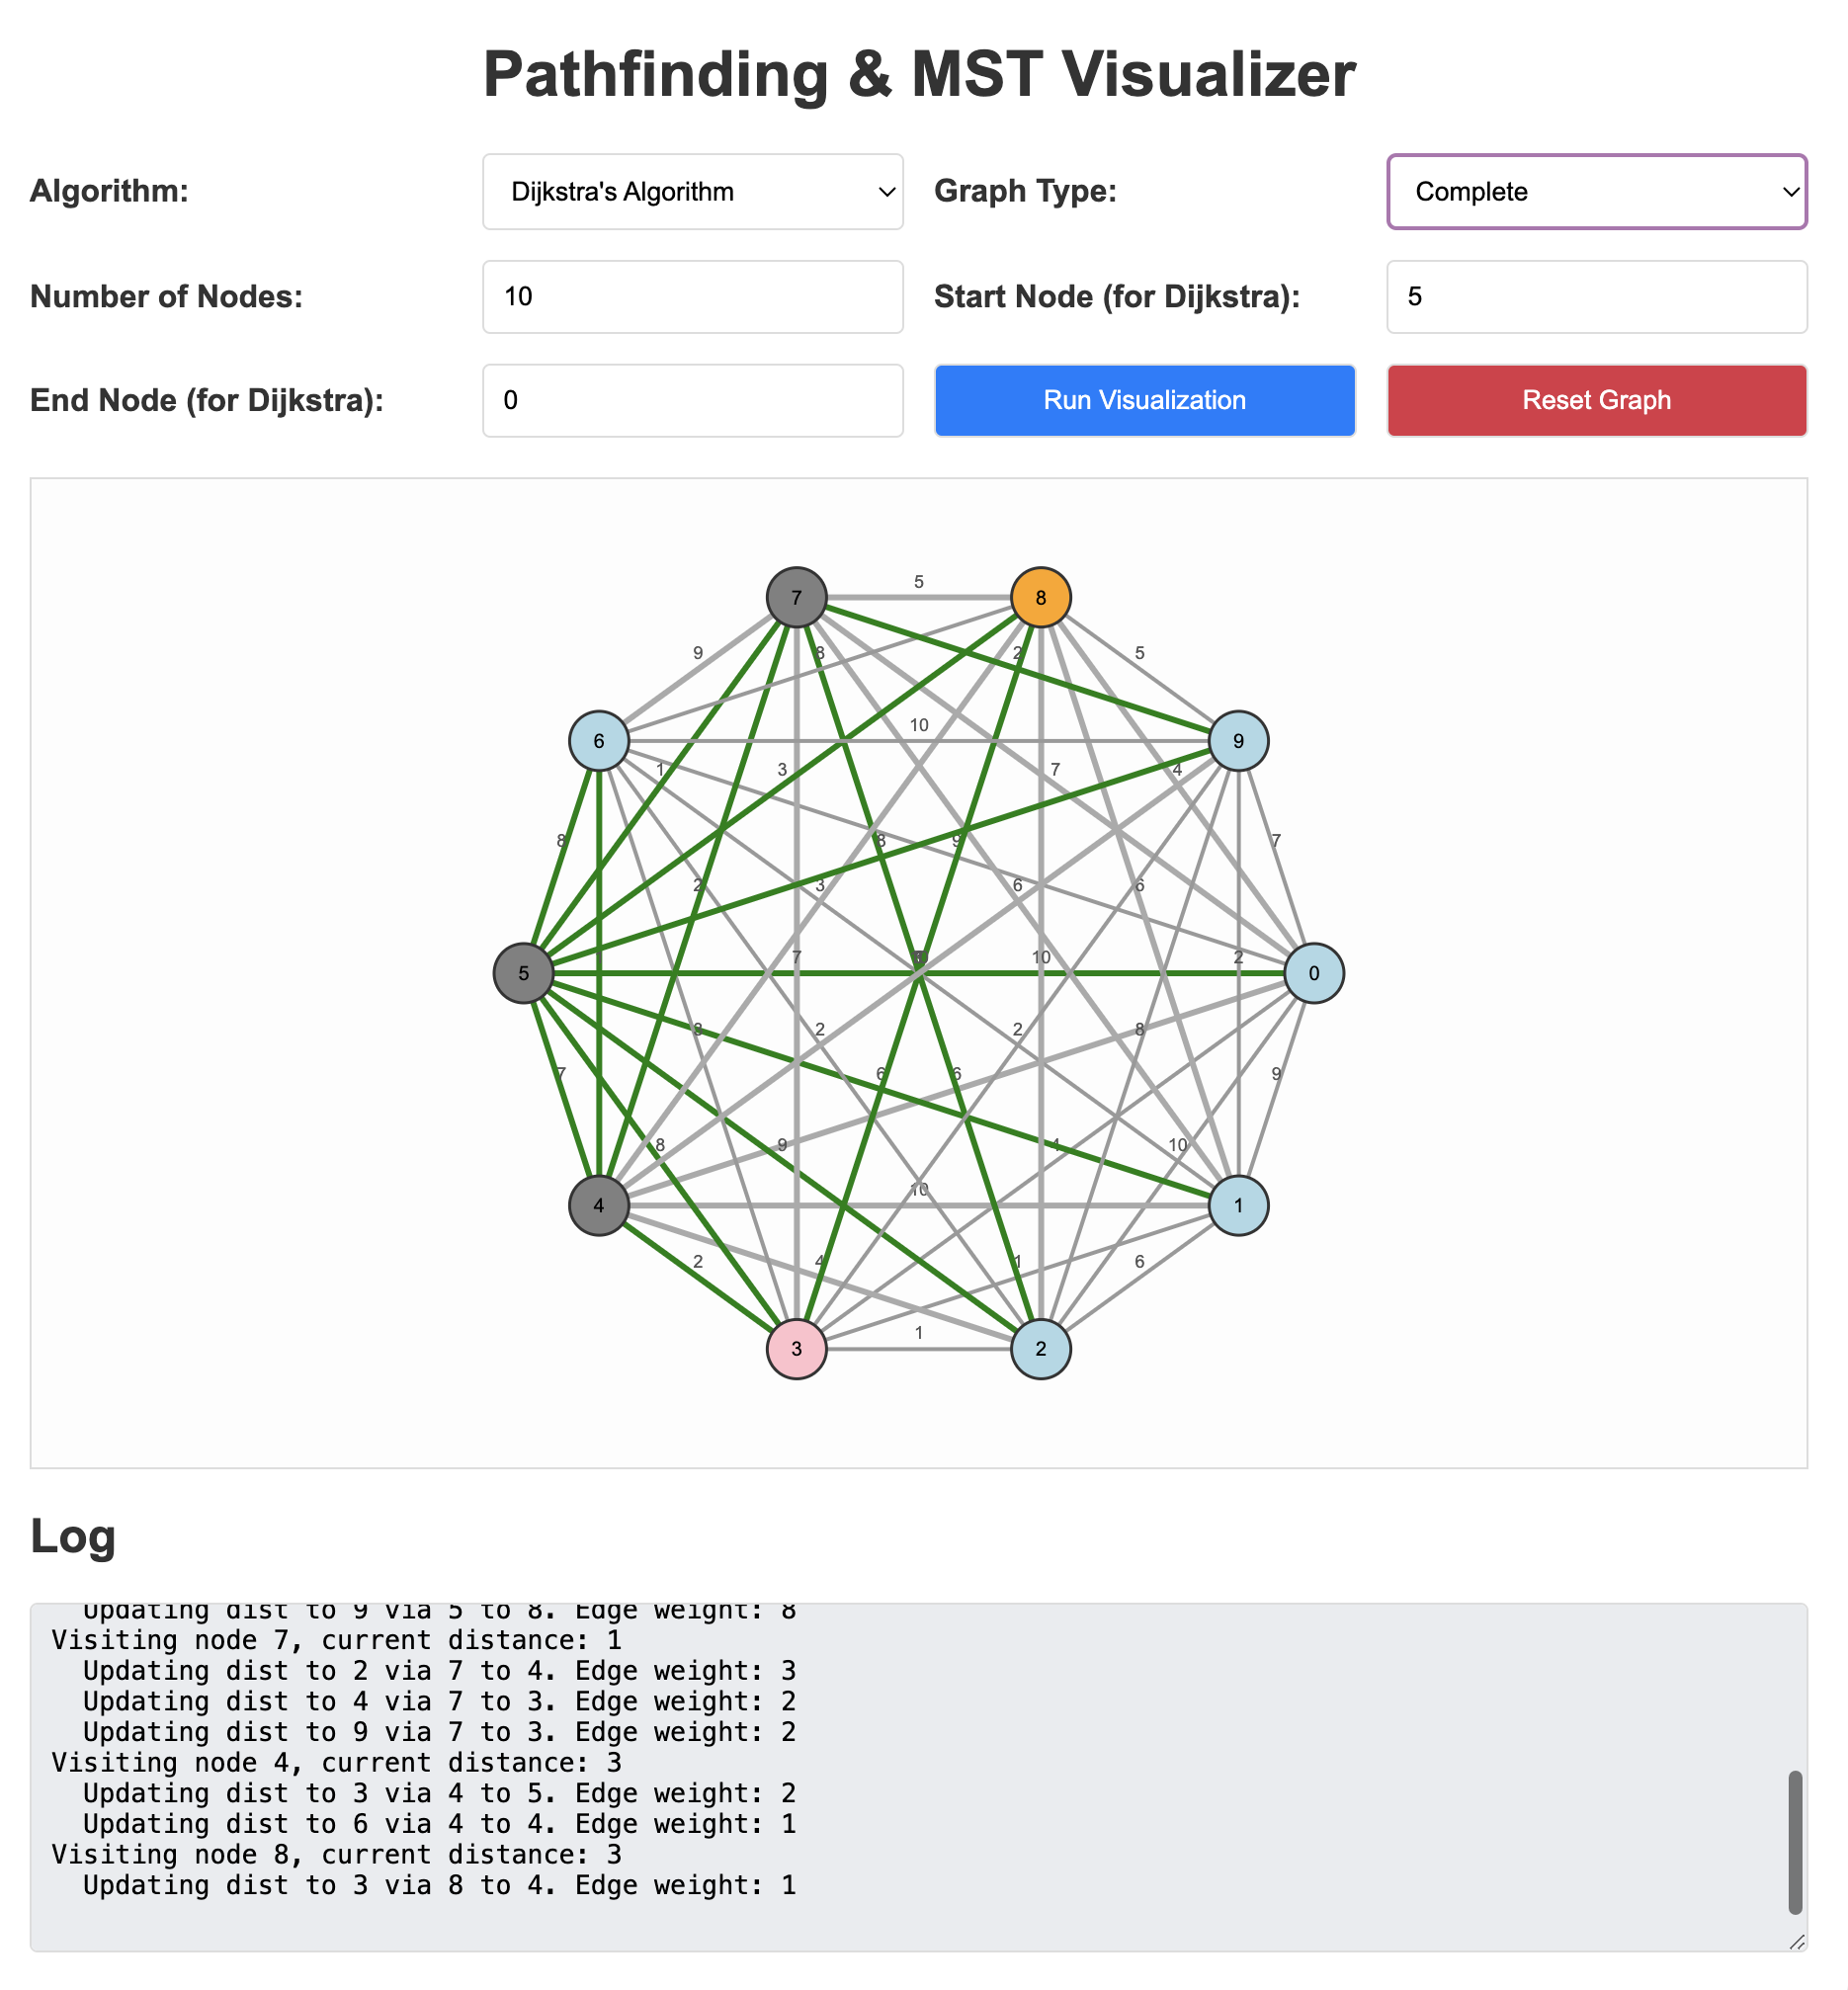
\includegraphics[width=0.9\textwidth]{images/all.png}
    \caption{Runtime comparison on different types of graphs ($d=0.8$)}
    \label{fig:all}
\end{figure}

\clearpage
\section*{Conclusion}
From our experiments:
\begin{itemize}
  \item \textbf{Prim's} performs better on dense graphs due to efficient heap operations on many edges.
  \item \textbf{Kruskal's} excels on sparse graphs where sorting fewer edges dominates less work in Union-Find.
\end{itemize}
Overall, for very large, dense graphs Prim’s is preferable; for large, sparse graphs, Kruskal’s is slightly faster.

This happens because of the approach that they use in path finding algorithm. For example Kruskal has a time complexity of 
$ O(E log(E)) $ because it sorts the graph only by the edge size. This is why on sparse graphs it performs better.
On the other hand Prim algorithm has a time complexity of $O(E log(V))$ where the number of edges has a lower influence

Also a good observation would be that in the visual example the Prim and Kruskal give the same spanning tree.
It's a common event if the weights of the graph are unique. If more edges hae the same weights, the Minimum 
Spanning Tree can be different.

\clearpage
\begin{thebibliography}{9}
  \bibitem{cormen} T.~H.~Cormen, C.~E.~Leiserson, R.~L.~Rivest, and C.~Stein, \emph{Introduction to Algorithms}, 3rd ed., MIT Press, 2009.
  \bibitem{kruskal} J.~B.~Kruskal, "On the shortest spanning subtree of a graph and the traveling salesman problem," \emph{PNAS}, vol.~7, no.~1, pp.~48--50, 1956.
  \bibitem{mstviz} MST Visualizer, \url{https://mst-visualizer.example.com}.
\end{thebibliography}
\end{document}
